\begin{document}
\chapter{Reti di Flusso}
Innanzi tutto inziamo con alcune definzioni:
\dfn{Rete}{
  definiamo \textbf{rete} un grafo \textit{pesato} $ G = (N,A) $ dove
  \begin{itemize}
    \item $ N $ e' l'insieme dei nodi
    \item $ A $ e' l'insieme degli archi
  \end{itemize}
}

Più precisamente:
\begin{itemize}
  \item $\forall i \in N$ è associato un valore reale $b_i$, detto \textit{sbilanciamento} che può essere:
  \begin{itemize}
    \item \textbf{Positivo}: il nodo $i$ è detto \textit{pozzo} e rappresenta la qunatità del bene che esce della rete al nodo $i$, mentre $b_i$ è ldetto \textit{domanda del bene}
    \item \textbf{Negativo}: il nodo $i$ è detto \textit{sorgente} e rappresenta la quantità del bene che entra nella rete al nodo $i$, mentre $-b_i$ è detto \textit{offerta del bene}
    \item \textbf{Nullo}: il nodo $i$ è detto \textit{transito} e rappresenta un nodo di passaggio
  \end{itemize}
  \item $\forall (i,j) \in A$ è associato un valore reale $c_{ij}$ detto \textit{costo} che rappresenta il costo di trasportare una unità di bene lungo l'arco $(i,j)$ ed una coppia di valori $l_{ij}$ e $u_{ij}$ detti \textit{capacità inferiore} e \textit{capacità superiore} rispettivamente, che rappresentano il minimo e il massimo numero di unità di bene che possono essere trasportate lungo l'arco $(i,j)$
  \begin{center}
    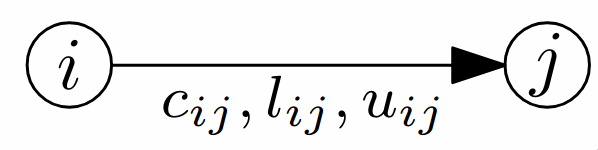
\includegraphics[width=0.5\textwidth]{img/2025-03-05-09-34-49.png}
  \end{center}
\end{itemize}

\section{Problemi di Flusso}
\dfn{Problemi di flusso}{
  > Si definiscono \textit{problemi di flusso} quei problemi che consistono nel determinare, lungo una rete, il flusso di un bene, ossia un assegnamento a ciascun arco \( (i,j) \in A \) un valore reale \( x_{ij} \in [l_{ij}, u_{ij}] \), rispettando i vincoli di capacità e conservazione del flusso
}

\textbf{flusso}, quindi, e' proprio la soluzione che vogliamo trovare. Tuttavia ad ogni unità di flusso assegnata ad un arco corrisponde un costo $c_{ij}$, si ha quindi che il costo complessivo del flusso e' dato da:
\begin{equation}  
  \sum_{(i,j) \in A} c_{ij}x_{ij}
\end{equation}


\subsection{Vincoli}
I vincoli che nei problemi di flusso si deve rispettare sono:
\begin{itemize}
\item \textit{Uguaglianza di domanda e offerta globale}:
  \begin{equation}
    \sum_{i \in D}b_i = - \sum_{i \in O} b_i \iff \sum_{i \in N} b_i = 0
  \end{equation}
  Dove $ D = \{b_i \in N \mid b_i > 0\} $ e $ O = \{b_i \in N \mid b_i < 0\} $. Per quelli nulli, tanto vale non metterli da nessuna parte per non creare asimmetria inutile.
\item \textit{Conservazione di flusso}:
  \begin{quote}
    lol 
    \hfill \textit{Il Basta}
  \end{quote}

  \begin{equation}
    \sum_{(i,j) \in BS(i)} x_{ij} - \sum_{(i,j) \in FS(i)} x_{ij} = b_i \quad \forall i \in N
  \end{equation}
  
dove
\begin{align*}
  BS(i) = \{(k,i) | (k,i) \in A\} \text{ detto stella entrante}\\
  FS(i) = \{(i,k) | (i,k) \in A\} \text{ detto stella uscente}
\end{align*}
Ovvero ciò che entra nel nodo e' uguale a cio' che esce piu' lo sbilanciamento.
\item \textit{Ammissibilità del flusso}:
  \[
    l_{ij} \leq x_{ij} \leq u_{ij} \quad \forall (i,j) \in A
  \]
\end{itemize}



\ex{Esempio di rete}{
  \begin{center}
    \begin{tikzpicture}[
        node distance=2cm,
        vertex/.style={circle, draw, minimum size=1cm},
        edge/.style={->, >=Stealth, auto},
    ]

    % Nodes
    \node[vertex] (1) {1};
    \node[vertex, below=of 1] (2) {2};
    \node[vertex, right=of 1] (3) {3};
    \node[vertex, below=of 3] (4) {4};

    % Edges
    \draw[edge] (1) -- node[above] {3, 1, 4} (3);
    \draw[edge] (1) -- node[left] {4, 0, 6} (2);
    \draw[edge] (2) -- node[below] {1, 2, 5} (4);
    \draw[edge] (3) -- node[right] {3, 1, 10} (4);

    % Labels
    \node[above left=0.1cm of 1] {3};
    \node[below left=0.1cm of 2] {4};
    \node[above right=0.1cm of 3] {2};
    \node[below right=0.1cm of 4] {5};

    \end{tikzpicture}
  \end{center}  
}

Perche' mai dovremmo studiare sta roba? 
\begin{itemize}
\item \textbf{Espressivita'}: permette di catturare un range di problemi concreti abbastanza grande
\item \textbf{Complessita'}: esistono algoritmi che risolvono questo tipo di problemi con complessita' polinomiale abbastanza basso. A Ugo questo fa molto piacere :), perché ricordiamolo NON SIAMO INGENERI GESTIONALI, SIAMO INFORMATICI
\end{itemize}

\subsection{Ipotesi semplificative}

Le ipotesi semplificative sono supposizioni che non consentono di usare il caso generale, ma che semplificano il problema \textbf{senza} perdere espressivita', come ad esempio nel caso in cui le capacita' inferiori sono nulle ovvero $l_{ij}=0$, che e' una situazione a cui possiamo arrivare \textbf{anche da grafi che non hanno questa caratteristica}. 

Infatti data una rete $G$, si può costruire una rete $G'$ tale che $G$ e $G'$ hanno lo stesso flusso ottimo, ma $G'$ ha capacita' inferiori nulle. $\forall (i,j)\in A$:
\begin{itemize}
\item Si sottrae $ l_{ij} $ a $ b_j $ e a $ u_{ij} $
\item Si aggiunge $ l_{ij} $ a $ b_i $
\item Occorre aggiungere la quantita'
  \[
    \sum_{(i,j) \in A} c_{ij}l_{ij}
  \]
  Alla funzione abbiettivo 
\end{itemize}
\nt{
  Si noti che non cambia la soluzione ottima, ma solo il valore ottimo della funzione obbiettivo
}

È pertanto vero, quindi, che ad un flusso $x_{ij} \in G $ corrisponde un flusso $(x_{ij}+l_{ij}) \in G'$
\subsection{Problema del Flusso di Costo Minimo}

\dfn{Problema del Flusso di Costo Minimo}{
  Si definisce \textit{problema del flusso di costo minimo} il problema di flusso in cui la funzione obbiettivo è il costo di flusso da minimizzare e le cui capacità inferiori sono nulle
}

Questo problema è formalizzabile in programmazione lineare come segue:
\begin{equation}
  \begin{aligned}
    \min &cx\\ 
    Ex &= b \quad \leq x \leq u  
  \end{aligned}
\end{equation}
dove

\begin{itemize}
  \item $x \in \mathbb{R}^{|A|} $ è il vettore delle variabili di flusso
  \item $c \in \mathbb{R}^{|A|} $ è il vettore dei costi
  \item $E \in \mathbb{R} ^{|N| \times |A|} $ e' una matrice di incidenza fra nodi e archi i cui elementi possono solo assumere valori 0, -1 e 1
  \item $b \in \mathbb{R}^{|N|} $ e' il vettore degli sbilanciamenti
  \item $u \in \mathbb{R}^{|A|}$ e' il vettore delle capacita' superiori
\end{itemize}

In questo modo abbiamo scritto funzione obbiettivo e vincola in forme matriciali molto semplici, adesso, senza terrorizzare nessuno, fornirò la formalizzazione in forma estesa:
\begin{equation}
  \begin{aligned}
    \min &\sum_{(i,j) \in A} c_{ij}x_{ij}\\
    &\sum_{(j,i)\in BS(i)}x_{ji} -\sum_{(i,j) \in A} x_{ij} = b_i \quad \forall i \in N\\
    &l_{ij} \leq x_{ij} \leq u_{ij} \quad \forall (i,j) \in A
  \end{aligned}
\end{equation}

\subsubsection{Rilassamento di assunzioni}
Puo' essere utile assumere che esiste un solo pozzo e una sola sorgente, che vengono poi collegati con archi fittizi (a costo nullo e capacita' pari allo sbilanciamento dei pozzi/sorgenti effettivi!) a quelli effettivi. 

Per trasformare un generico problema MCF in un problema con una sola sorgente ed un solo pozzo$ \dots $
\begin{itemize}
  \item Si aggiungono due nodi fittizi $s$ e $t$, uno sorgente e uno pozzo
  \item Si aggiungono archi fittizi  da $s$ ai nodi sorgenti di partenza, con un costo nullo e capacita' pari all'inverso dello sbilanciamento del nodo sorgente, ovvero $-b_s$
  \item Si aggiungono archi fittizi dai nodi pozzo ai nodi pozzo di arrivo, con un costo nullo e capacita' pari allo sbilanciamento del nodo pozzo
  \item Lo sbilanciamento di $s$ e' pari alla somma degli sbilanciamenti dei nodi sorgenti, mentre lo sbilanciamento di $t$ e' pari alla somma degli sbilanciamenti dei nodi pozzo
\end{itemize}

\ex{Esempio di Rilassamento}{
  Si parte da questa rete:
  \begin{center}
    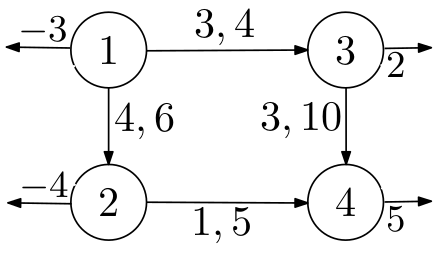
\includegraphics[width=0.5\textwidth]{img/rete_non_rilassata.png}
  \end{center}
  Si aggiungono i nodi fittizi $s$ e $t$ con sbilanciamento rispettivamente $b_s =b_1+b_2=-3-4 =-7$ e $b_t = b_3+b_4 = 2+5 =7$

  Si aggiungono gli archi fittizi con costo nullo e con capacità:
  \begin{itemize}
    \item $a_{s1} = -b_1 = 3$
    \item $a_{s2} = -b_2 = 4$
    \item $a_{3t} = b_3 = 2$
    \item $a_{4t} = b_4 = 5$
  \end{itemize}

  Si ottiene quindi la seguente rete rilassata:
  \begin{center}
    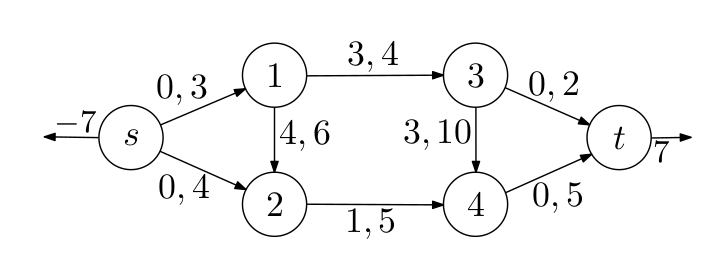
\includegraphics[width=0.5\textwidth]{img/rete_rilassata.png}
  \end{center}
}
\begin{quote}
  Non si può, però, enunciare che i nodi non hanno una capacita', perche' di fatto non succede nulla, perche' puo' essere trasformata in una rete equivalente dove i nodi non ce l'hanno:

  \hfill \textit{TODO: spiegare meglio, che cazzo vuoi dire ibbastianini?}

  Mi spiego in modo piu' eloquente: Per poter utilizzare nodi che hanno una propria capacita', non e' necessario perdere generalita' cambiando la definizione del problema esaminato. Questo e' vero, in quanto una tale rete puo' essere banalmente trasformata in una rete equivalente la quale presenta solo nodi con capacita' nulla. Come accade tale trasformazione? Facciamocelo spiegare da GioPalmi:
\end{quote}

Alle volte, inoltre, è utile che anche i nodi abbiano delle \textbf{capacità}, ossia che solo che solo una quantità di flusso compresa nell’intervallo chiuso $[l_i , u_i]$ possa passare per il nodo $i \in N$. Per fare ciò occorre \textit{sdoppiare} ciascun nodo $i$ in due nodi $i',i''$, in modo che:
\begin{itemize}
  \item Tutti gli archi entranti in $i$ entrino in $i'$ 
  \item tutti gli archi uscenti da $i$ escano da $i''$
  \item Si aggiunge un arco da $i'$ a $i''$ con capacità $[l_i,u_i]$
\end{itemize}
\begin{center}
  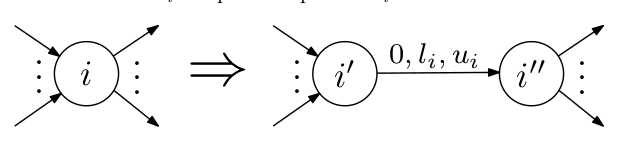
\includegraphics[width=0.5\textwidth]{img/giga_archetto_con_capacity.png}
\end{center}

\subsection{Problema di Flusso Massimo}

\dfn{Problema di Flusso Massimo}{
  Dato un grafo $ G = (N,A) $ orentato su cui definiamo:
  \begin{itemize}
  \item il vettore di capacita' superiori $ u = [u_{ij}] $ associate agli archi
  \item $ s $ (\textit{origine} o \textit{sorgente}) e $ t $ (\textit{destinazione} o \textit{pozzo}) due nodi distinti
  \end{itemize} 
  si definisce \textit{problema di flusso massimo} il problema di massimizzazione del flusso da $ s  $ a $ t $.

  Ovvero, il problema consiste nel trovare il \textbf{massimo} valore $ v $ tale che se $ b_s = -v $, $ b_t = v $ e per tutti gli altri casi $ b_i = 0 $, allora esiste un flusso $ x = [x_{ij}] $ ammissibile. Tale $ v $ si dice \textbf{valore} del flusso $ x $.
}
Ciò che cambia, quindi, dal problema di flusso di costo minimo è la funzione obbiettivo, che diventa, si vuole infatti \textit{massimizzare} il flusso, e non minimizzare il costo (che non ci interessa). 

Formalizzato in programmazione lineare, il problema di flusso massimo diventa:
\begin{equation} \label{PL_FM}
  \begin{aligned}
  \max \quad & v \\
  \sum_{(j,s) \in BS(s)} x_{js} + v &= \sum_{(s,j) \in FS(s)} x_{sj}; \\
  \sum_{(j,i) \in BS(i)} x_{ji} - \sum_{(i,j) \in FS(i)} x_{ij} &= 0, \quad i \in N - \{s, t\}; \\
  \sum_{(j,t) \in BS(t)} x_{jt} &= \sum_{(t,j) \in FS(t)} x_{tj} + v; \\
  0 \leq x_{ij} &\leq u_{ij}, \quad (i,j) \in A.
  \end{aligned}
\end{equation}

\nt{
  Si noti che il problema di flusso massimo e' un caso particolare di problema di flusso di costo minimo. Difatti la formulazione \ref{PL_FM} puo' essere vista come la descrizione di un problema di MCF su un grafo $ G' $ ottenuto da $ G $ con delle modifiche: 
  \begin{itemize}
    \item Si aggiunge un arco fittizio $ (t,s) $, detto \textit{arco di ritorno}, con capacita' infinita.
    \item Tutti i nodi sono di trasferimento ($ \forall i \in N.\ b_i = 0 $), si tratta quindi di un problema di \textit{circolazione}.
    \item Tutti i costi degli archi sono nulli tranne $ (t,s) $ che ha costo $ -1 $.
  \end{itemize}

  Di conseguenza, risolvendo il problema di MCF su $ G' $, stiamo minimizzando il valore $ -1 \cdot x_{ts} $ rispettando i vincoli imposti, che per definizione corrisponde a $ -v $. Ma minimizzare $ -v $ significa massimizzare il valore $ v $ del flusso fra $ t $ ed $ s $, che  e' proprio l'obbiettivo del problema di MF.
}

\ex{Risolvere un problema MF come MCF}{ \label{ex:FM}
  Dato il seguente problema di MF, con capacita' superiori indicate in figura e dove i nodi diversi da $ s $ e $ t $ hanno sbilanciamento nullo (come per definizione del problema), trasformarlo in un problema MCF:
  \begin{center}
    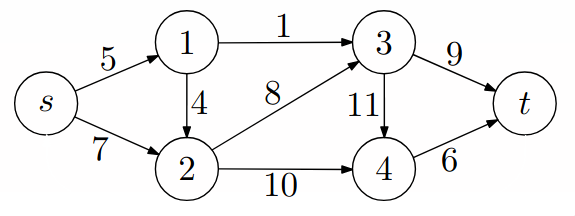
\includegraphics[width=0.5\textwidth]{img/2025-03-13-11-01-34.png}
  \end{center}

  Il problema di MF consiste nel determinare il massimo valore di flusso $ v $, ovvero il massimo valore di sbilanciamento uguale per $ s  $ (ma con segno meno) e $ t $ (devono essere per forza uguali per il vincolo di \textit{uguaglianza di domanda e offerta globale}) per cui esiste un flusso ammissibile $ x = [x_{ij}] $ (che quindi rispetta i vincoli di \textit{ammissibilita'} e di \textit{conservazione}). 

  A prima occhiata, possiamo subito dire che il valore limite per $ v $ e' sicuramente $ 5 + 7 = 12 $, dato che per il vincolo di conservazione $ b_s = x_{s1} + x_{s2} \leq u_{s1} + u_{s2} $ (facendo lo stesso ragionamento con $ t $, otteniamo un limite meno stringente, quindi prevale questo). Siamo sicuri che $ v = 0 $ sara' sempre una soluzione ammissibile, dato che $ x = \underline{0} $ e' sempre un flusso ammissibile, ma non e' quasi mai il valore massimo. Facciamo i passi con $ v = 12 $:
  \begin{itemize}
  \item Dobbiamo mettere $ x_{s1} = 5 $ e $ x_s2 = 7 $
  \item Dobbiamo mettere $ x_{13} = 1 $ e $ x_{12} = 4 $
  \item Ora abbiamo che $ \sum_{(j,i) \in BS(2)} x_{ji} = 7 + 4 = 11 $ e dobbiamo decidere come dividere il flusso entrante fra quelli uscenti, dato che questa volta non vengono saturati. Possiamo usare l'euristica e guardare i nodi di destinazione: il 3 ha capacita' superiori per i flussi uscenti rispetto al nodo 4, quindi gli mandiamo piu' flusso possibile (questa e' solo un'intuizione e non e' affatto una regola generale). Quindi $ x_{23} = 8 $ e $ x_{24} = 3 $.
    \item Poniamo $ x_{3t} = 9 $ e $ x_{4t} = 3 $: esiste un flusso $ x $ ammissibile per $ v = 12 $! E dato che 12 e' il limite massimo, siamo sicuri che e' la soluzione al problema.
  \end{itemize}

  Non sempre sara' cosi' facile trovare la soluzione corretta. Vediamo il problema MCF corrispondente e convinciamoci che e' equivalente:
  \begin{center}
    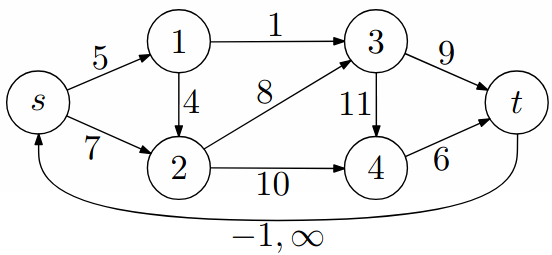
\includegraphics[width=0.5\textwidth]{img/2025-03-13-11-38-15.png}
  \end{center}

Le capacita' massime sono uguali, tutti i nodi hanno sbilanciamento nullo e abbiamo aggiunto l'arco di ritorno. La funzione obbiettivo e:
\[
min -x_{ts} \equiv max x_{ts}
\]
dato che tutti gli altri costi sono nulli. Dato che $ s  $ e $ t $ hanno sbilanciamento nullo, per i vincoli di conservazione e di ammissibilita':
\[
x_{ts} = x_{3t} + x_{4t} \leq u_{3t} + u_{4t} = 15 \quad \land \quad u_{s1} + u_{s2} = 12 \geq x_{s1} + x_{s2} = x_{ts}
\]
da qui otteniamo che $ x_{ts} \leq 12 $ e' il limite superiore. Da questo punto, controllare se con $ x_{ts} = 12 $ possiamo costruire un flusso ammissibile segue lo stesso identico procedimento di prima. Quindi il flusso che minimizza il costo e' proprio $ x $ il cui valore di flusso associato $ v = x_{ts} $ e' il valore della soluzione MF.
}
  
\section{Problema del flusso massimo: algoritmi}
Abbiamo capito quindi che il problema di Flusso Massimo e' un problema di MCF con due caratteristiche specifiche:
\begin{itemize}
\item Il vettore dei bilanci $ b $ e' nullo
\item Il vettore dei costi $ c $ e' nullo tranne per $ c_{ts} $ che vale $ -1 $
\end{itemize}
Vediamo come queste caratteristiche permettono di utilizzare algoritmi specifici al problema, che sono molto piu' veloci di quelli generali.

\subsection{Tagli}

\dfn{Taglio}{
  Si definisce \textbf{taglio} in una rete $G=(N,A)$ una coppia $(N',N'')$ di sottoinsiemi di $N$ tali che $N' \cup N'' = N$ e $N' \cap N'' = \emptyset$
}

Si noti, inoltre anche questa defnizione
\dfn{$(s,t)$-taglio}{
  Si definisce \textbf{$(s,t)$-taglio} in una rete $G=(N,A)$ un taglio ($N_s, N_t$) dove $s \in N_s$ e $t \in N_t$
}

Si prendi in considerazione inoltre i confini il confine fra gli $(s,t)-\text{tagli}$, dove:
\begin{itemize}
  \item $A^+(N_s, N_t) = \{(i,j) \in A \mid i \in N_s \land j \in N_t\}$ sono gli archi che vanno dalla partizione $s$ a $t$
  \item $ A^-(N_s,N_t)=\{(i,j)\in A\mid i\in N_t\land j\in N_s\} $ sono gli archi che vanno da $t$ a $s$
\end{itemize}

\ex{Taglio (s,t) di un problema di flusso massimo}{
  Ecco un esempio di taglio (rappresentato dalla riga blu) che partiziona in due sottoinsiemi i nodi di un problema di flusso massimo:
  \begin{center}
    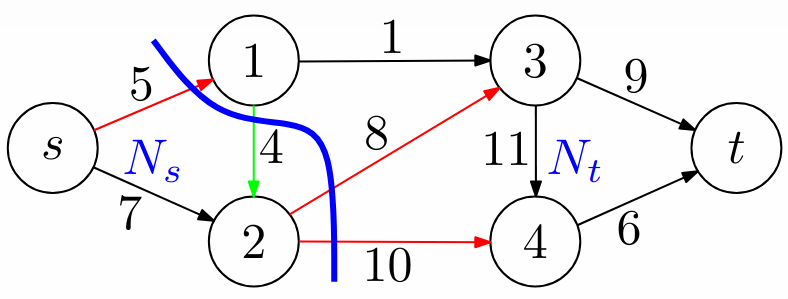
\includegraphics[width=0.5\textwidth]{img/2025-03-13-18-25-02.png}
  \end{center}
  Dal grafo si deduce che:
  \begin{itemize}
  \item $ N_s = \{s,2\} $
  \item $ N_t = \{1,3,4,t\} $
  \item $ A^{+} = \{(s,1), (2,3), (2,4)\} $
  \item $ A^{-} = \{(1,2)\} $
  \end{itemize}
}

Adesso introduciamo un importante lemma sui tagli:
\mlenma{}{
  $\forall (s,t)-\text{taglio }(N_s,N_t)$ e $\forall$ flusso ammissibile $x$ con valore $v$, si ha che:
  \begin{itemize}
    \item $v = \sum_{(i,j)\in A^+(N_s,N_t)}x_{ij}- \sum_{(i,j)\in A^-(N_s,N_t)}x_{ij}$
    
    Si ha, quindi, che $v$ la somma del flusso uscente da $s$ meno il flusso entrante in $s$.     Questa quantità è detta \textbf{flusso del taglio} $(N_s, N_t)$ e la si denota $x(N_s, N_t)$

    \item $v\leq \sum_{(i,j)\in A^+(N_s, N_t)} u_{ij}$
    
    Ovvero Il flusso massimo è sempre minore o uguale alla capacità totale del taglio. Questa quantità è detta \textbf{capacità del taglio} ed è indicata con $u(N_s, N_t)$
  \end{itemize}
}
\pf{Dimostrazione}{
  \begin{itemize}
    \item Dimostro la prima parte:
    Per definizione di $v$, si ha che:
    \[
      v = \sum_{(s,j)\in A}x_{sj} - \sum_{(i,s)\in A}x_{is}
    \]
    
      
    Questo valore è uguale alla somma netta in uscita $\forall i\in N_s$ verso la partizione $N_t$, quindi:
      \footnote{
        Possiamo dimostrare questa cosa dato che, per il vincolo di conservazione e per definizione del problema:
      \[
        \forall k \in N_s.\ \sum_{(k,j) \in A} x_{kj} - \sum_{(i,k)} x_{ik} = \begin{cases}
        v & k = s \\
        0 & k \neq s 
        \end{cases}
      \]
      }
    \[
      \sum_{(i,j)\in A}x_{ij} - \sum_{(i,j)\in A}x_{ji} = \sum_{k\in N_s}\left( \sum_{(k,j)\in A}x_kj-\sum_{(i,k)\in A}x_{ik} \right)
    \]
    Riscrivendo usando la proprieta' distributiva, posso dividere l'esspressione in due parti:
      \[
        \underbrace{\sum_{k \in N_s} \sum_{(k,j) \in A} x_{kj}}_\text{somma archi uscenti $ S^{+} $} - 
        \underbrace{\sum_{k \in N_s} \sum_{(i,k)} x_{ik}}_\text{somma archi entranti $ S^{-} $}
      \]
      Dato che $ k \in N_s $, consideriamo tutti gli archi $ (p,q) $ che hanno \textit{almeno} un nodo dentro a $ N_s $, ci sono quindi tre casi:
      \[
      \begin{cases}
        p \in N_s \land q \in N_t & \to S^{+} \mathrel{+}= x_{pq} \\
        p \in N_t \land q \in N_s &  \to S^{-} \mathrel{+}= x_{pq} \\
        p,q \in N_s & \to S^{+} \mathrel{+}= x_{pq} \land S^{-} \mathrel{+}= x_{pq}
      \end{cases}
      \]
      Ma aggiungere lo stesso valore in $ S^{+} $ e in $ S^{-} $ non ha effetto sul valore finale dato che si annullano, quindi possiamo anche non considerare gli archi fra nodi che appartengono a $ N_s $. 

      Consideriamo quindi solo gli archi che attraversano il taglio: $ S^{+} $ e' la somma dei flussi da $ N_s $ a $ N_t $ e $ S^{-} $ i flussi da $ N_t $ a $ N_s $. Quindi la loro somma e' uguale al flusso uscente dal confine $A^+(N_s, N_t)$ meno il flusso entrante dal confine $A^-(N_s, N_t)$, allora:
    \[
      \sum_{k\in N_s}\left( \sum_{(k,j)\in A}x_kj-\sum_{(i,k)\in A}x_{ik} \right) = \sum_{(i,j)\in A^+(N_s,N_t)}x_{ij}- \sum_{(i,j)\in A^-(N_s,N_t)}x_{ij}
    \]
  
    Per riassumere quindi:
    \begin{equation}
      v = \sum_{(i,j)\in A^+(N_s,N_t)}x_{ij}- \sum_{(i,j)\in A^-(N_s,N_t)}x_{ij}
    \end{equation}
    \item Dimostro la seconda parte:
    
    Ovvio perché è una semplice derivazione del punto 1
  \end{itemize}
}

\nt{
  si noti che la conclusione di questo Lemma è
  \[
    v = x(N_s, N_t)\leq u (N_s, N_t)
  \]

  Ovvero \textit{il valore di un flusso ammissibile è sempre minore o uguale della capacità di qualunque taglio}. 
}
\nt{
  Abbiamo utilizzato il secondo punto del lemma all'esempio \ref{ex:FM}, quando abbiamo imposto un limite superiore al valore di $ v $ sommando le capacita' massime degli archi uscenti da $ s  $ e poi con gli archi entranti a $ t $. Quindi e' come se avessimo costruito un taglio con $ N_s = \{s \} $ e uno con $ N_t = \{t\} $, per poi imporre il secondo punto del lemma, scegliendo quello minore come limite. 

  Pero' abbiamo controllato solo due tagli specifici, quello che aggiunge il lemma e' che tale proprieta' vale per tutti i tagli, quindi per trovare un limite migliore tocca calcolare la capacita' di tutti i tagli possibili.
}

Adesso tratteremo il caso un cui si voglia determinare se esiste un taglio con capacità \textbf{identica} al valore di un flusso ammissibile (ovvero massimo)

\subsection{Cammini aumentanti e Grafo residuo}
Innanzi tutto dobbiamo presentare alcuni concetti


\subsubsection{Cammino aumentante}
Dato una rete di un problema di MF e un suo flusso ammissibile, noi vogliamo sapere se questo flusso e' ottimo. Se non fosse ottimo, cio' significa che sarebbe possibile inviare altro flusso da $ s $ a $ t $, che quindi dovra' seguire un certo cammino $ P $. Tale cammino non segue per forza l'orientamento del grafo, quindi e' possibile che un arco $ (i,j) $ venga attraversato al contrario. Provo a dare l'intuizione del perche' con un esempio:
\ex{}{
  Consideriamo il seguente grafo (ignorare il taglio):
  \begin{center}
    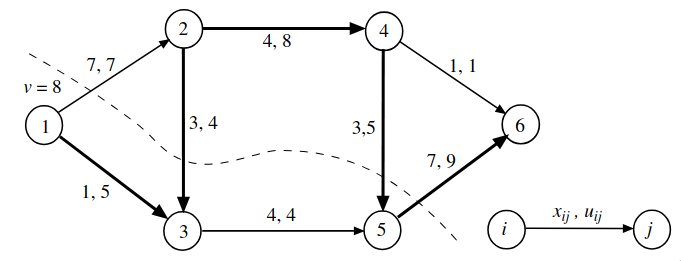
\includegraphics[width=0.5\textwidth]{img/2025-03-13-21-24-42.png}
  \end{center}
  Attualmente, il valore del flusso vale 8. Vogliamo vedere se e' possibile aumentare il flusso. Proviamo ad aumentare il flusso di 2 ($ v = 10 $):
  \begin{itemize}
    \item Dato che l'arco $ (1,2) $ e' saturo, devo aumentare $ x_{13} $ di 2
    \item L'unico arco uscente da 3 e' saturo, quindi non possiamo far proseguire il flusso. Puo' sembrare di essere in un vicolo cieco, perche' dove lo mettiamo questo flusso in piu'? Ma, come abbiamo detto prima, il cammino che stiamo cercando \textit{non e' per forza orientato}, quindi sarebbe possibile "proseguire" lungo l'arco $ (2,3) $ al contrario. Questo e' perche' in questa situazione possiamo fare una giocata: il nodo 3 e' sovraccaricato, dato che il flusso non puo' uscire da nessuna parte, quindi dobbiamo diminuire quello in entrata. Il flusso $ x_{13} $ appena aumentato lo vogliamo tenere, dato che fa parte del percorso, quindi \textit{diminuiamo} il flusso $ x_{12} $ della stessa quantita' di quanto abbiamo aumentato il flusso dell'arco entrante. In questo modo il totale di flussi entranti al nodo 3 rimane uguale, ma il nodo 2 ha ora ben 2 di flusso in piu' che puo' utilizzare! Quindi, il flusso in piu' che vogliamo far arrivare a 6 si e' spostato da 3 a 2, ed e' proprio per questo che possiamo attraversare gli archi al contrario. Ma attenzione, al posto di aumentare il valore del flusso $ x_{23} $, l'abbiamo diminuito, cosa che definiremo meglio dopo.
    \item Ora che il nodo 2 ha del flusso extra, lo inviamo al nodo 4 ($ x_{24} += 2 $)
    \item Il nodo 4 lo manda al nodo 5 che infine lo manda al nodo 6.
  \end{itemize}
  Notare che se avessimo scelto di aumentare $ v $ di 3, dal nodo 4 non sarebbe stato possibile rispettare i vincoli di ammissibilita', quindi il valore 2 non era scelto a caso.
}

Ora che e' chiaro cosa stiamo cercando e perche', iniziamo a formalizzare le intuizioni. Per prima cosa, distinguiamo gli archi attraversati col verso "giusto" da quelli attraversati con verso "opposto":
\dfn{Archi concordi e discordi}{
  Dato un cammino $ P $ su una rete $ G $, chiamiamo:
  \begin{itemize}
  \item L'insieme degli archi \textit{conocrdi} $ P^{+} $ l'insieme degli archi del percorso $ P $ che hanno lo stesso orientamento degli archi corrispondenti in $ G $
  \item L'insieme degli archi \textit{discordi} $ P^{-} $ l'insieme degli archi del percorso $ P $ che hanno verso opposto rispetto agli archi corrispondenti in $ G $
  \end{itemize}
}

\ex{}{
  Quindi, nell'esempio di prima:
  \begin{itemize}
    \item $ P^{+} = \{(1,3), (2,4), (4,5), (5,6)\} $
    \item $ P^{-} = \{(3,2)\} $
  \end{itemize}
}

Definiamo ora la capacita' di un percorso, che dimostreremo essere la quantita' in piu' di flusso che tale percorso puo' portare da $ s  $ a $ t $:
\dfn{Capacità di un cammino}{
  Dato un cammino $P$ in una rete $G$ rispetto a un flusso $x$, la \textbf{capacità} di $P$ rispetto a $x$ è definita come:
  \begin{equation}
    \theta (P,x) = \min{\{\min{\{u_{ij}-x_{ij}\mid (i,j)\in P^+\}},\min{\{x_{ij}\mid (j,i)\in P^-\}}\}}
  \end{equation} 
}

\nt{
  Quindi abbiamo definito $ \theta(P,x) $ in questo modo per fare in modo che corrisponda alla quantita' massima di flusso che possiamo mandare in piu' rispetto al flusso OG $ x $ in modo che rimanga sempre ammissibile. Notare che e' possibile che tale valore sia nullo, nel caso in cui uno degli archi concordi e' saturo o uno di quelli discordi e' nullo, in questo caso $ P $ non e' aumentante.
}

Dalla definizione di capacita' discende la definizione di flusso $x(P,\theta)$:
\dfn{Flusso $x(P,\theta)$}{
  Dato un cammino aumentante $P$ in una rete $G$ rispetto a un flusso $x$ e una capacità $\theta$, il flusso $x(P,\theta)$ è definito come:
  \begin{equation}
    (x(P,\theta))_{ij} = 
    \begin{cases}
      x_{ij}+\theta & (i,j)\in P^+\\
      x_{ij} - \theta & (i,j)\in P^-\\
      x_{ij} & \text{altrimenti}
    \end{cases}
  \end{equation}
}

\mlenma{}{
  Se $ x $ e' ammissibile, allora anche $ x(P, \theta(P, x)) $ e' ammissibile
}
\pf{}{
  TODO: dimostra (facile)
}

Possiamo ora definire un cammino aumentante come:
\dfn{Cammino aumentante}{
  Data una rete $ G $ di un problema MF, un cammino da $ s  $ a $ t $ \textit{non necessariamente orientato} si dice \textbf{aumentante} se $ \theta(P,x) > 0 $.
}

\subsubsection{Grafi residui}

Per definire un algoritmo che riesca a determinare se esisti o meno un cammino aumentante dato un grafo $ G $ e un flusso ammissibile $ x $, ci e' piu' comodo lavorare su sul cosidetto \textit{grafo residuo} $ G_x $ associato: 
\dfn{
  grafi residui
}{
  Dati una rete $G =(N_G, A_G)$ ed un flusso ammissibile $x$ si definisce il \textbf{grafo residuo} $G_x$ il multigrafo $(N_{G_x}, A_{G_x})$ tale che:
  \begin{itemize}
    \item $N_{G_x} = N_G$
    \item Gli archi in $A_{G_x}$ sono di due tipi:
    \begin{itemize}
      \item $\forall (i,j)\in A_G$ tale che $x_{ij}<u_{ij}$ esiste un arco da $i$ a $j$ in $G_x$ detto \textbf{arco concorde}
      
      Signifca che il flusso non ha saturato la capicità dell'arco e si può ancora inviare flusso in quella direzione
      \item $\forall (i,j)\in A_G$ tale che $x_{ij}> 0$ esiste un arco da $j$ a $i$ in $G_x$ detto \textbf{arco discorde}
    \end{itemize}
  \end{itemize}
}

\nt{
  Osserviamo come in $A_{G_x}$ ci possano essere al piu' due archi per ogni arco $ (i,j) \in A_{G} $ (uno concorde e l'altro discorde), quindi se in $ A_{G} $ esistono gli archi $ (i,j) $ e $ (j,i) $, e' possibile che in $ A_{G_x} $ ci siano due archi $ (i,j) $ e due archi $ (j,i) $ con capienze diverse.
}

Introduciamo ora due lemmi che legano i cammini aumentanti di $ G $ a cammini semplici e orientati in questo nuovo grafo:
\mlenma{}{
  Per ogni cammino aumentante da $ s  $ a $ t $ rispetto a $ x $ in $ G $, esiste uno ed un solo cammino \textit{orientato} da $ s $ a $ t $ in $ G_x $.
}
\pf{}{
  Per come abbiamo costruito il grafo residuo $ G_x $, $ \forall (i,j) \in A $ se l'arco non e' saturo, allora esiste l'arco orientato $ (i,j) \in A_x $ che puo' far parte degli archi \textit{conocordi} di un cammino aumentante. Se l'arco $ (i,j) \in A $ e' non nullo, allora esiste l'arco orientato in modo opposto $ (j_x, i_x) \in A_x $, che puo' fare parte degli archi \textit{discordi} di un cammino aumentante.

  Quindi, se esiste un cammino aumentante $ P $ su $ G $ dato $ x $, allora e' possibile seguire un cammino semplice orientato da $ s  $ a $ t $ sul grafo dei residui $ G_x $, proprio perche' sappiamo che se $ P $ e' aumentante allora tutti gli archi che percorre saranno non saturi (se attraversti in modo orientato) e non nulli (se attraversati in modo opposto), quindi esisteranno per forza i corrispondenti archi orientati in $ G_x $.
}
\mlenma{}{
  Se $ G_x $ non ha cammini semplici orientati da $ s  $ a $ t $, allora $ x $ e' un flusso massimo.
}
\pf{}{
  Sappiamo che $ x $ e' un flusso massimo di valore $ v $ se determiniamo un taglio $ (N_s, N_t) $ la cui capacita' e' pari a $ v $ (TODO: introdurre e dimostrare prima questo lemma). Ci riduciamo quindi a dimostrare che esiste un tale taglio sul grafo residuo $ G_x $ se questo non ha visite che raggiungono $ t $.

  Siano $ N_s $ tutti i nodi raggiungibili da $ s  $ in $ G_x $ e $ N_t = N \setminus N_s $ i restanti (contiene almeno $ t $ per ipotesi). Siccome non ci sono archi che collegano nodi da $ N_s $ a $ N_t $, significa che nel grafo $ G $ tutti gli archi di $ A^{+}(N_s, N_t) $ sono saturi e tutti gli archi di $ A^{-}(N_s, N_t) $ sono nulli, altrimenti ci sarebbe stato almeno un arco in $ G_x $ che collega $ N_s $ a $ N_t $.

  Quindi il flusso del taglio (che equivale al valore del flusso $ x $ per il lemma) avra' il valore:
  \[
    x(N_s, N_t) = v = \underbrace{\sum_{(i,j) \in A^{+}} x_{ij}}_\text{saturo} 
    - \underbrace{\sum_{(i,j) \in A^{-}} x_{ij}}_\text{nullo} = \sum_{(i,j) \in A^{+}} u_{ij} = u(N_s, N_t)
  \]
  Abbiamo quindi dimostrato il lemma.
}

\nt{
  In altre parole, l'ultimo lemma ci dice che se non esistono cammini aumentanti su $ G $ per un dato flusso $ x $, allora nel grafo $ G_x $ non esistono cammini semplici orientati da $ s  $ a $ t $.
}

Quindi per torvare un cammino aumentante, basta far partire una visita da $ s  $ nel grafo $ G_x $ e vedere se $ t $ e' raggiungibile!

\subsubsection{Note}
Volendo, era possibile partire dalla definizione:
\dfn{Cammino aumentante (usando $ G_x $)}{
  Un \textbf{cammino aumentante} $P$ in un grafo residuo $G_x$ è un cammino semplice e orientato da $s$ a $t$.
}
Nelle slide e' cosi', ma penso che sia piu' corretto partire dal concetto di cammino aumentante sul grafo $ G $ (che e' piu' intuitivo) per poi mostrare l'equivalenza con un cammino orientato sul suo grafo residuo.


\subsection{Algoritmo Ford-Fulkerson}

Miglioriamo il flusso corrente usando il grafo residuo con cammino aumentante. Quindi visitiamo il grafo residuo partendo da s, e se c'e' un cammino che arriva a t significa che e' aumentante, quindi si aggiorna x il meglio possibile. fare questo finche non si trova il cammino aumentante, quindi abbiamo ottimizzato :)

\begin{algorithm}
  \caption{Algoritmo di Ford-Fulkerson}
  \KwIn{Grafo $G$ con sorgente $s$ e sink $t$}
  \KwOut{Flusso massimo $x$}

  $x \gets 0$\;

  \While{True}{
    Make($G_x$)\tcp*{Costruisci il grafo residuo $G_x$}
    \If{$\exists$ un cammino aumentante $P\in G_x$}{
      $x \gets x(P, \theta(P, x))$\;
    }
    \Else{
      \Return $x$\;
    }
  }
\end{algorithm}

TODO: usa lemmi dati in precedenza per dimostrare che sta roba funzia

\subsection{Algoritmo di Edmonds-Karp}
L'algoritmo di Ford-Fulkerson è corretto ma può avere complessità esponenziale nel caso pessimo. L'algoritmo di Edmonds-Karp nasce proprio per rendere la complessità di Ford-Fulkerson polinomiale nel caso pessimo, l'idea è mantenere quindi l'algoritmo invariato, ma cambiare il modo in cui si scelgono i commini aumentanti nel grafo residuo $G_x$, imponendo che la ricerca del cammino aumentante venga fatta usando \textbf{BFS (Breadth - First Search)}

\nt{
  Grazie alla visita in ampiezza i cammini aumentanti saranno sempre cammini di lunghezza minima
}

\subsubsection{Correttezza}

EK è trivialmente 

\subsubsection{Complessità}

Per valutarne la complisstià occorre procedere in questo modo, prima si procede osservando che, se in FF i cammini aumentanti sono di lunghezza minima, allora la distanza di un generico nodo $i$ dalla sorgente $s$ in $G_x$ non può diminuire, da ciò si deducie che il numero di iterazione di EK non può essere asintoticamnte più grande di $N\cdot A$. In particolare:

\dfn{Distanza fra nodi di un grafo residuo}{
Data una rete $G$, un flusso ammissibile $x$ e due nodi $i,j$ in $G$, indiachiamo con $\delta_x (i,j)$ la distanza tra $i$ e $j$ nel grafo residuo $G_x$
}
\mlenma{}{ \label{lem:BK_distAum}
  Se, durante l'esecuzione di EK il flusso $y$ è ottenuto da $x$ tramite un’operazione di aumento del flusso in un cammino aumentante, allora per ogni nodo $i \in N$ , vale che
  \[
    \delta_x (s, i) \leq \delta_y (s, i)
  \]
}

\pf{}{
  oH
}

\thm{Teorema sulla complessità di Edmonds-Karp}{
  Il numero di iterazioni di EK è $O(N A)$, quindi la sua complessità è $O(N A^2)$
}

Prima della dimostrazione si noti questa definizione
\dfn{arco critico}{
  Un arco $(i,j)$ è detto \textbf{critico} per un cammino aumentante $P$ se la sua capacità (ossia $u_{ij}-x_{ij}$ se è concorde o $x_{ji}$ se è discorde) è uguale a $\theta(P,x)$
}
\nt{
  In ongi cammino aumentante, esiste almeno un arco critico (e ce ne possono essere piu' di uno). Sono quindi gli archi che spariscono quando viene aggiunto $ \theta(P, x) $.
}

\dimostrazione{
  Si procede nel contare quante volte un arco $(i,j)$ può diventare critico prima di scomparire definitivamente da grafo
  \begin{itemize}
    \item Quando $(i,j)$ diventa critico per la prima volta significa che nel grafo residuo:
    \[
      \delta_x (s,j) = \delta_x (s,i)+1
    \]
      Cioè, $j$ si trova a distanza 1 in più di $i$ dalla sorgente nel BFS.\footnote{Questo e' perche' stiamo usando proprio la BFS, che garantisce che $ (s,i) $ e' un cammino minimo per arrivare a $ i $ e che il nodo $ j $ sia sicuramente piu' lontano da $ s  $ rispetto a $ i $ (altrimenti il cammino aumentante non passerebbe da $ i $). Quindi, dato che $ i $ e $ j $ sono collegati, il cammino minimo per arrivare da $ s  $ a $ j $ non sara' maggiore di $ \delta_x(s,i) + 1 $ e deve essere che $ \delta_x(s,j) \geq \delta_x(s,i) $. Dato che la distanza e' un numero intero, l'unico valore ammissibile e' questo.}
    \item Perché $(i,j)$ possa \textbf{riapparire} nel grafo residuo, deve succedere che il flusso da $i$ a $j$ diminuisca+
    , cioè:
    \begin{equation}
        \delta_y(s, i) = \delta_y(s, j) + 1
    \end{equation}
      Ma allora, per il lemma \ref{lem:BK_distAum}:
    \begin{equation}
        \delta_y(s, i) = \delta_y(s, j) + 1 \geq \delta_x(s, j) + 1 = \delta_x(s, i) + 2
    \end{equation}
    \textbf{Quindi la distanza da $s$ aumenta di almeno 2} ogni volta che un arco diventa critico di nuovo.
    
    \item \textbf{Limite massimo sul numero di volte in cui un arco può diventare critico}:
    \begin{itemize}
        \item La distanza di un nodo da $s$ nel BFS \textbf{non può superare} $|N|$ (il numero di nodi).
        \item Poiché la distanza aumenta \textbf{di almeno 2} ogni volta che $(i,j)$ diventa critico, un arco può essere critico \textbf{al più $O(N)$ volte}.
    \end{itemize}

  \end{itemize}
}

\subsection{Algoritmo di Goldberg-Tarjan}

Un'altro approccio possibile che permette di scendere sotto la soglia di una complessità $O(V\,A^2)$ consiste nell'utilizzare sempre un algoritmo iterativo, ma locale rispetto al grafo, in quanto il flusso viene modificato solo in una parte del grafo (in opposizione con FF ed EK, in cui ad ogni iterazione occorre procedere con un’analisi globale), un concetto fondamentale che sta dietro all'algoritmo è il concetto di \textbf{preflusso}

\dfn{preflusso}{
  Un \textbf{preflusso} è un vettore $x$ tale che:
  \begin{equation}
    \sum_{(j,i)\in BS(i)} x_{ji}-\sum_{(i,j)\in BS(i)}x_{ij}\geq 0, \quad i\in N\backslash \{s,t\}
  \end{equation}

  In altre parole, i vincoli di capacità sono soddisfatti, al contrario, quelli di bilanciamento possono non esserlo. \textbf{ciò che entra in un nodo è $\geq$ a quello che esce}. 
}
\nt{
  Usiamo questa definizione di flusso piu' "lasca" dato che modificamndo il flusso di un arco solo difficilmente porta ad un flusso totale ammissibile.
}

che è collegato all'idea di nodo attivo
\dfn{nodo attivo/bilanciato}{
  Un nodo si dice \textbf{attivo} se il suo eccesso
  \begin{equation}
    e_i = \sum_{(j,i)\in BF(i)} x_{ji}- \sum_{i,j}x_{i,j}
  \end{equation}
}

L'idea centrale dell'algoritmo è quella di eliminare gli sbilanciamenti presenti nel prefusso corrente. In altre parole cercando di rendere i nodi attivi in nodi bilanciati in modo eliminando l'eccedenza "spostandola" verso i nodi più vicini, in modo \textit{iterativo} e \textit{locale}.

Lo sbilanciamento presente in un nodo i viene eliminato spostando parte del flusso in eccesso, mediante due diverse azioni
\begin{itemize}
  \item \textbf{push forward}: viene in avanti, ossia attraverso un arco $(i, j)$, ogniqualvolta $x_{ij} < u_{ij}$ (quindi se $x_{ij}$ ha capacità residua)
  \item \textbf{backward.}: viene in avanti, ossia attraverso un arco $(j, i)$, ogniqualvolta $x_{ij} > 0$
\end{itemize}

Tuttavia queste operazioni di push non possono essere sempre eseguite per evitare situazioni di loop o di complessità troppo elevata. Si utilizza un sistema di etichettature: intuitivamente si può trasferire del flusso in avanti o in dietro sse il nodo i ha un'altitudine (una quota) maggiore rispetto agli altri nodi verso i quali si vuole trasferire del flusso (1 o 0)

Adesso fornirò l'algoritmo 
\begin{algorithm}
  $x\gets 0$\;
  $x_{sj} \gets u_{sj} \forall(s, j) \in FS (s)$\tcp*{Faccio uscire tutto quello che posso da s, quindi, quello che esce da s è almeno pari al massimo}
  $d\gets EtichettaturaValida(G)$\;
  $d_s \gets n$\tcp*{la quota di esse assume il numero di nodi della rete}
  \If{$\forall N\in G\backslash \{s,t\}, N$ è bilanciato}{
    \Return $x$
  }
  \ForEach{$N \in G: N$ sbilanciato}{
    $v\gets N$\;
    \If{$\exists (v,j)\text{ ammissibile per }v$}{
      $PushForward(v, j)$\;
    }
    \If{$\exists (i,v)$ ammissibile per $v$}{
      $PushBackward(i, v)$\;
    }
    $Relabel(v)$\;
  }
\end{algorithm}
\subsubsection{Correttezza e complessità}
\thm{}{
  L’algoritmo di Goldberg e Tarjan è corretto, e la sua complessità in tempo è $O(N^2 A)$ 
}

\section{Il Problema del Flusso di Costo Minimo: Algoritmi}
\subsection{nozioni preliminari}
La teoria dei cammini minimi successivi si trasmette bene da problemi di flusso massimo a problemi di costo minimo. Grafi residui e capacita' rimangono uguali, ma e' diverso come determinimao il cammino aumentante di costo minimo dato che dobbiamo tenere in consideraizone il costo.

Partiamo con la definizione di pseudoflusso
\dfn{pseudoflusso}{
  Uno \textbf{pseudoflusso} è un vettore $x$ che soddisfa i vincoli di capacità, ossia tale che
  \begin{equation}
    0\leq x_{ij}\leq u_{ij}\quad (i,j)\in A
  \end{equation}
}
Da cui discende 
\dfn{sbilanciamento}{
  Se $x$ è uno pseudoflusso, definiamo sbilanciamento di un nodo $i$ rispetto a $x$ la quantità
  \begin{equation}
    e_x(i) = \sum_{(j,i)\in BS(i)} x_{ji} - \sum_{(i,j)\in FS(i)}x_{ij}- b_i
  \end{equation}

  In pratica $e_x(i)$ può essere visto come un vettore degli sbilanciamenti
}
Il nostro abbiettivo sarà trasformare lo pseudoflusso in un'altro pseudoflusso che risolva le "anomalie" del flusso di partenza, queste anomalie sono dei valori molto alti nel vettore di sbilanciamento

\dfn{}{
  Si ha inoltre che dato uno pseudoflusso $x$, i nodi sbilanciati rispetto a $x$ fanno parte di uno dei seguenti due insiemi 
\[
  \begin{aligned}
    O_x &= \{i\in N\mid e_x (i)> 0\} \text{ quindi lo sbilanciamento è strettamente positivo}\\
    D_x &= \{i\in N \mid e_x (i) < 0\} \text{ quindi lo sbilanciamento è strettamente positivo}
  \end{aligned}
\]
I nodi in $O_x$ sono detti \textbf{nodi con eccesso di flusso}, mentre quelli in $D_x$ sono detti \textbf{nodi con difetto di flusso}

}

  Con $O_x$ si va a segnalare che ciò che entra è inferiore a ciò che esce, al contrario $D_x$
\nt{
  Si noti che che se $O_x = N_x = \emptyset$ si ha che $x$ è un flusso, si può quindi intuire che occorrerà procedere sbarazzandoci di $O_x$ e $D_x$
}

Un indice ancora più precise che indica quanto è lontano uno pseudoflusso con un flusso ammissibile è:

\dfn{sbilanciamento complessivo}{
  Lo \textbf{sbilanciamento complessivo} di x è definito come:
  \begin{equation}
    g(x) = \sum_{i\in O_x} e_x (i) = - \sum_{j\in D_x} e_x(j)
  \end{equation}
}

\subsection{Cammini aumentanti}
Per introdurre concetti futuri occorre "generalizzare" il concetto di grafi residui e cammini aumentanti, si ha che:
\dfn{grafo residuo per pseudo flusso}{
  Si definisce \textbf{grafo residuo per uno pseudoflusso} $x$ il grafo residuo $G_x$ definito in precedenza dove ogni arco ha un costo:
  \begin{itemize}
    \item $\forall (i,j)\in G_x$ il costo è $c_{ij}$
    \item $\forall (i,j)\in G_x$ il costo è $-c_{ij}$
  \end{itemize}
}
Poi si definisce il cammino aumentate 
\dfn{cammino aumentante}{
  Un \textbf{cammino aumentante} $P$ tra $i$ e $j$ in $G_x$ è un cammino semplice nell'arco residuo (tra $i$ e $j$)
}

ovviamente i suoi archi possono essere partizionati in $P^+$ e $P^-$ e la sua capiacità $\delta(P,x)$ è definita come al solito

\dfn{ciclo aumentante}{
  un cammino aumentante tra $i$ e $j$ viene anche detto \textbf{ciclo aumentante}
}

  Vorremmo quindi utilizzare questi cammini aumentati per diminuire lo sbilanciamento 

  Dato uno pseudoflusso x e un cammino aumentante P , è
  possibile inviare $0 \leq \theta \leq \theta(P, x)$ (capacità residua lungo un cammino $P$) unità di flusso lungo attraverso l’operazione $x(P, \theta)$, denoteremo in questo contesto $ x(P, \theta) $ (il flusso che ottengo da x pompando $\theta$ unità di flusso lungo $P$) verrà spesso indicato anche con $x \oplus P \theta$. Se P è un cammino aumentante da i a j in Gx , allora lo pseudoflusso $x(P, \theta)$ avrà gli stessi sbilanciamenti di x, tranne in i e $j$, infatti se io amunto il flusso che va da $i$  a $j$, tutti gli sbilanciamenti tutti i nodi non cuivolti rimarrano tali e quali, nei nodi che sono attraversati dal cammino tra i e j, ciò entrerà nei nodi sara la setessa quantità di ciò che uscire per definizione dell'operazione di update, ciò che entra viene aumentato e ciò che esce viene aumentato. pertanto lo sbilanciamento avrà solo effetti tra $i$ e $j$ (se sono uguali il vettore degli sbilanciamenti sarà inalterato). Si passi adesso alla def di costo
  \dfn{
    costo
  }{
    il costo di un cammino aumentate $P$ è definito come \begin{equation}
      c(P) = \sum_{(i,j)\in P^+}c_{ij} - \sum_{(i,j)\in P^-}c_{ij}
    \end{equation}
  }
  Si verifica facilmente che 
  \[
    c · (x(P, \theta)) = c · (x \oplus P \theta) = c · x + \theta c(P )
  \]


\thm{struttura degli Psudoflussi}{
    Siano x e y due pseudoflussi qualunque. Allora esistono $k \leq  n + m$ cammini aumentanti P1 , . . . , Pk , tutti per x, di cui al più m sono cicli, tali che:
    \begin{equation}
      \begin{aligned}
        z1 = x\\
    z_{i+1} = zi \oplus \theta i Pi\\
    z_{k+1} = y \quad 1\leq i\leq k\\
    0 \leq  \theta_i \leq  \theta(P_i , z_i )\\
      \end{aligned}
    \end{equation}
Inoltre, tutti i Pi hanno come estremi dei nodi in cui lo
sbilanciamento di x è diverso da quello di y.
  }

\subsection{minimalità}
\dfn{pseudoflusso minimale}{
  si definisce pseduofluddo minimale è uno pseudoflusso x che
  abbia costo minimo tra tutti gli pseudoflussi aventi lo stesso
  vettore di sbilanciamento ex
}

Occorre tra gli algoritmi che vedremo preservare la minimalità evitando di aumentare il costo flusso indiscriminatamente, Un problema centrale è quindi quello di determinare quali
siano le operazioni di aumento lecite e quali siano le
proprietà sui flussi che esse garantiscano.

\mlenma{}{Uno pseudoflusso (rispettivamente, un flusso ammissibile) è
minimale (rispettivamente, ottimo) sse non esistono cicli
aumentanti di costo negativo}
\pf{Dimostrazione}{
  \begin{itemize}
    \item $\Rightarrow$ Per contrapposizione: se esiste un ciclo aumentante di costo negativo in
    $G_x$, applicarlo fa diminuire il costo senza alterare lo sbilanciamento, in
    contraddizione con la minimalità di $x$.

    \item $\Leftarrow$ Ancora per contrapposizione: supponiamo che $x$ non sia minimale,
    ossia che esista $y$ con $c_y < c_x$ e $e_y = e_x$. Allora per il teorema sugli
    pseudoflussi possiamo scrivere $y = x \oplus \theta_1 P_1 \oplus \ldots \oplus \theta_n P_n$, dove $\theta_i > 0$
    e ciascun $P_i$ è un ciclo. Da $c_y < c_x$ discende però che:
    \[
      c_x > c_x + \theta_1 c(P_1) + \ldots + \theta_n c(P_n)
    \]
    e quindi, è ovvio, che $c(P_i) < 0$ per qualche $i$.
\end{itemize}
}

Si può inoltre dimostrare un altro teorema
\thm{}{
  Sia $x$ uno pseudoflusso minimale e sia $P$ un cammino
aumentante rispetto ad $x$ avente costo minimo tra tutti i
cammini che uniscono un nodo di $O_x$ ad un nodo di $D_x$. Allora,
qualunque sia $\theta \leq \theta(x, P)$, abbiamo che $x(\theta, P) = x \oplus \theta P$ è
ancora pseudoflusso minimale.



}
\pf{Dimostrazione}{
  \begin{itemize}
    \item Siano $s$ e $t$ i vertici che $P$ collega. Supponiamo che $\theta \leq \theta(x, P)$ e che $y$
    sia un qualunque pseudoflusso con vettore di sbilanciamento $e_{x(\theta, P)}$.
    \item Per il Teorema sulla struttura degli pseudoflussi esistono:
    \begin{itemize}
        \item $k$ cammini aumentanti $P_1, \ldots, P_k$ rispetto a $x$, tutti da $s$ a $t$;
        \item $h$ cicli aumentanti $C_1, \ldots, C_h$ rispetto a $x$.
    \end{itemize}
    tali che $y = x \oplus \theta_1 P_1 \oplus \ldots \oplus \theta_k P_k \oplus \mu_1 C_1 \oplus \ldots \oplus \mu_h C_h$, (dove tutti gli
    $\theta_i, \mu_j$ sono positivi).
    \item Deve essere, per ragioni che hanno a che fare con lo sbilanciamento,
    che $\sum_{1\leq i \leq k} \theta_i = \theta$.
    \item Poiché $x$ è minimale, $c(C_i) \geq 0$.
    \item Siccome $P$ ha costo minimo, $c(P_i) \geq c(P)$.
    \item Di conseguenza:
    \[
    cy = cx + \theta_1 c(P_1) + \ldots + \theta_k c(P_k) + \mu_1 c(C_1) + \ldots + \mu_h c(C_h) \geq cx + \theta c(P) = cx(\theta, P).
    \]
\end{itemize}

}

\section{Problemi di Accoppiamento}
\begin{itemize}
\item \textbf{Accoppiamento di Massima Cardinalita'}
\item \textbf{Accoppiamento di Costo Minimo}
\end{itemize}

\subsection{Massima Cardinalita'}
Possiamo vederlo come un problema di flusso massimo con piu' sorgenti e piu' pozzi (ma questo l'abbiamo gia risolto). Bisogna un po' riflettere su come attribuire le capacita', in questo caso abbiamo due valori: 0 o 1 (non sceglere o scegliere). 

Ogni volta che abbiamo un flusso ammissibile intero, abbiamo un accoppiamento. Dato che non abbiamo flussi frazionari, la proprieta' di unico arco e' rispettata perche' sarebbe impossibile avere un grafo bilanciato con piu' archi per nodo. 


Il valore massimo teorico sara' $ min \{|O|, |D|\} $, dato che non hanno necessariamente la stessa cardinalita'. Non e' necessario usare EK, dato che non c'e' il rischio delle situaizoni patologiche che rallentano FF. 

\subsection{Costo Minimo}
In questo caso, vediamo il problema come uno di flusso di costo minimo, dove i nodi in O hanno sbilanciamento -1 e quelli in D 1, dove ogni arco ha un certo costo 
\end{document}
